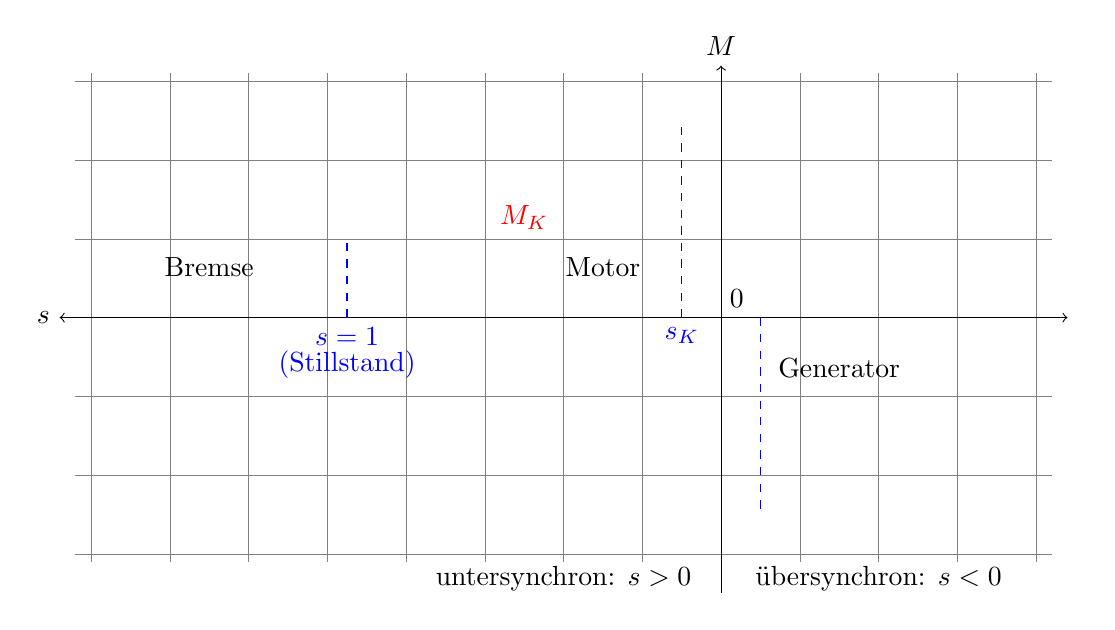
\begin{tikzpicture}[domain=-16:8, samples=200]
				\draw[very thin,color=gray] (-8.2,-3.1) grid (4.2,3.1);
				\draw[<->] (-8.4,0) node[left] {$s$} -- (4.4,0) node[right] {$\varPhi$};
				\draw[->] (0,-3.5) -- (0,3.2) node[above] {$M$};
				\draw[color=red, scale=1/2, smooth] plot[id=klossche_kennlinie] function{-5 * (2 / (x / 0.96 + 0.96 / x))} node[right] {};
				\draw (0.2,0) node[above] {$0$};
				\draw[color=red] (-2.5,1) node[above] {$M_K$};
				\draw[dashed, color=blue] (-0.5,0) node[below] {${s_K}$} -- (-0.5,2.5);
				\draw[dashed, color=blue] (0.5,0) node[above] {} -- (0.5,-2.5);
				\draw[dashed, color=blue] (-4.75,0) node[below] {${s = 1}$} -- (-4.75,1);
				\draw[color=blue] (-4.75,-0.3) node[below] {(Stillstand)};
				\draw (-6.5,0.4) node[above] {Bremse};
				\draw (-1.5,0.4) node[above] {Motor};
				\draw (1.5,-0.4) node[below] {Generator};
				\draw (-2,-3.6) node[above] {untersynchron: $s > 0$};
				\draw (2,-3.6) node[above] {übersynchron: $s < 0$};
				\end{tikzpicture}